% =========================================================
\section{I. Giới Thiệu Đồ Án \& Mục Tiêu}
% =========================================================

% SLIDE 2: Bối Cảnh & Vấn Đề
\begin{frame}
\frametitle{Bối Cảnh \& Vấn Đề}
\begin{itemize}
    \item \textbf{Xu hướng hiện nay:} Trỗi dậy của dòng game "Suy luận xã hội" (\textit{Social Deduction}), điển hình như \textit{Among Us, Goose Goose Duck}.
    \item \textbf{Nhu cầu:} Người chơi khao khát sự kết nối, tương tác và "lừa lọc" vui vẻ với nhau.
    % \item \textbf{Tình hình thực tế:}
    % \begin{itemize}
    %     \item Các game \textit{Saboteur} trên thị trường chủ yếu là \textbf{2D tĩnh}.
    %     \item Thiếu không khí "tụ tập" và tương tác vật lý trong môi trường chơi.
    % \end{itemize}
    
    \item \textbf{Game bài trong Game:} Các trò chơi kinh điển như \textbf{Uno, Mèo nổ, Ma sói} đã chứng minh sức hút mãnh liệt khi được số hóa, tạo ra cộng đồng hàng triệu người chơi.
\end{itemize}
\vspace{0.5cm}
    Do đó, nhóm đã chọn đề tài phát triển một trò chơi dạng Suy luận xã hội và Party kết hợp với game bài.
\end{frame}

\begin{frame}
\frametitle{Các Game Tiêu Biểu Trên Thị Trường}
\begin{columns}
    \column{0.6\textwidth}
    \textbf{Sự Thành Công Của Dòng Game Social \& Party:}
    
    \begin{itemize}
        \item \textbf{Among Us (Social Deduction):}
        \begin{itemize}
            \item Trở thành hiện tượng toàn cầu với lối chơi suy luận đơn giản nhưng kịch tính.
            \item Thành công nhờ tạo ra các tình huống tương tác xã hội "dở khóc dở cười".
        \end{itemize}
         
    \end{itemize}
    \vspace{6em}

    \column{0.4\textwidth}
    \centering
    
    \begin{figure}
        \centering
        
\includegraphics[width=0.8\linewidth]{img/amongus.png}
        % \caption{Enter Caption}
        \label{fig:amongus}
    \end{figure}
\end{columns}
\end{frame}

\begin{frame}
\frametitle{Các Game Tiêu Biểu Trên Thị Trường}
\begin{columns}
    \column{0.6\textwidth}
    \textbf{Sự Thành Công Của Dòng Game Social \& Party:}
    
    \begin{itemize}
        \item \textbf{Among Us (Social Deduction):}
        \begin{itemize}
            \item Trở thành hiện tượng toàn cầu với lối chơi suy luận đơn giản nhưng kịch tính.
            \item Thành công nhờ tạo ra các tình huống tương tác xã hội "dở khóc dở cười".
        \end{itemize}
        
        \item \textbf{Liar's Bar (Psychological Tabletop):}
        \begin{itemize}
            \item Gây sốt nhờ kết hợp sự căng thẳng của trò chơi "Bluffing" với môi trường 3D sống động.
            \item Đạt thành công lớn trong việc mô phỏng áp lực tâm lý giữa những người chơi trực tiếp.
        \end{itemize}
        
    \end{itemize}
    \vspace{3em}

    \column{0.4\textwidth}
    \centering
    
    \begin{figure}
        \centering
        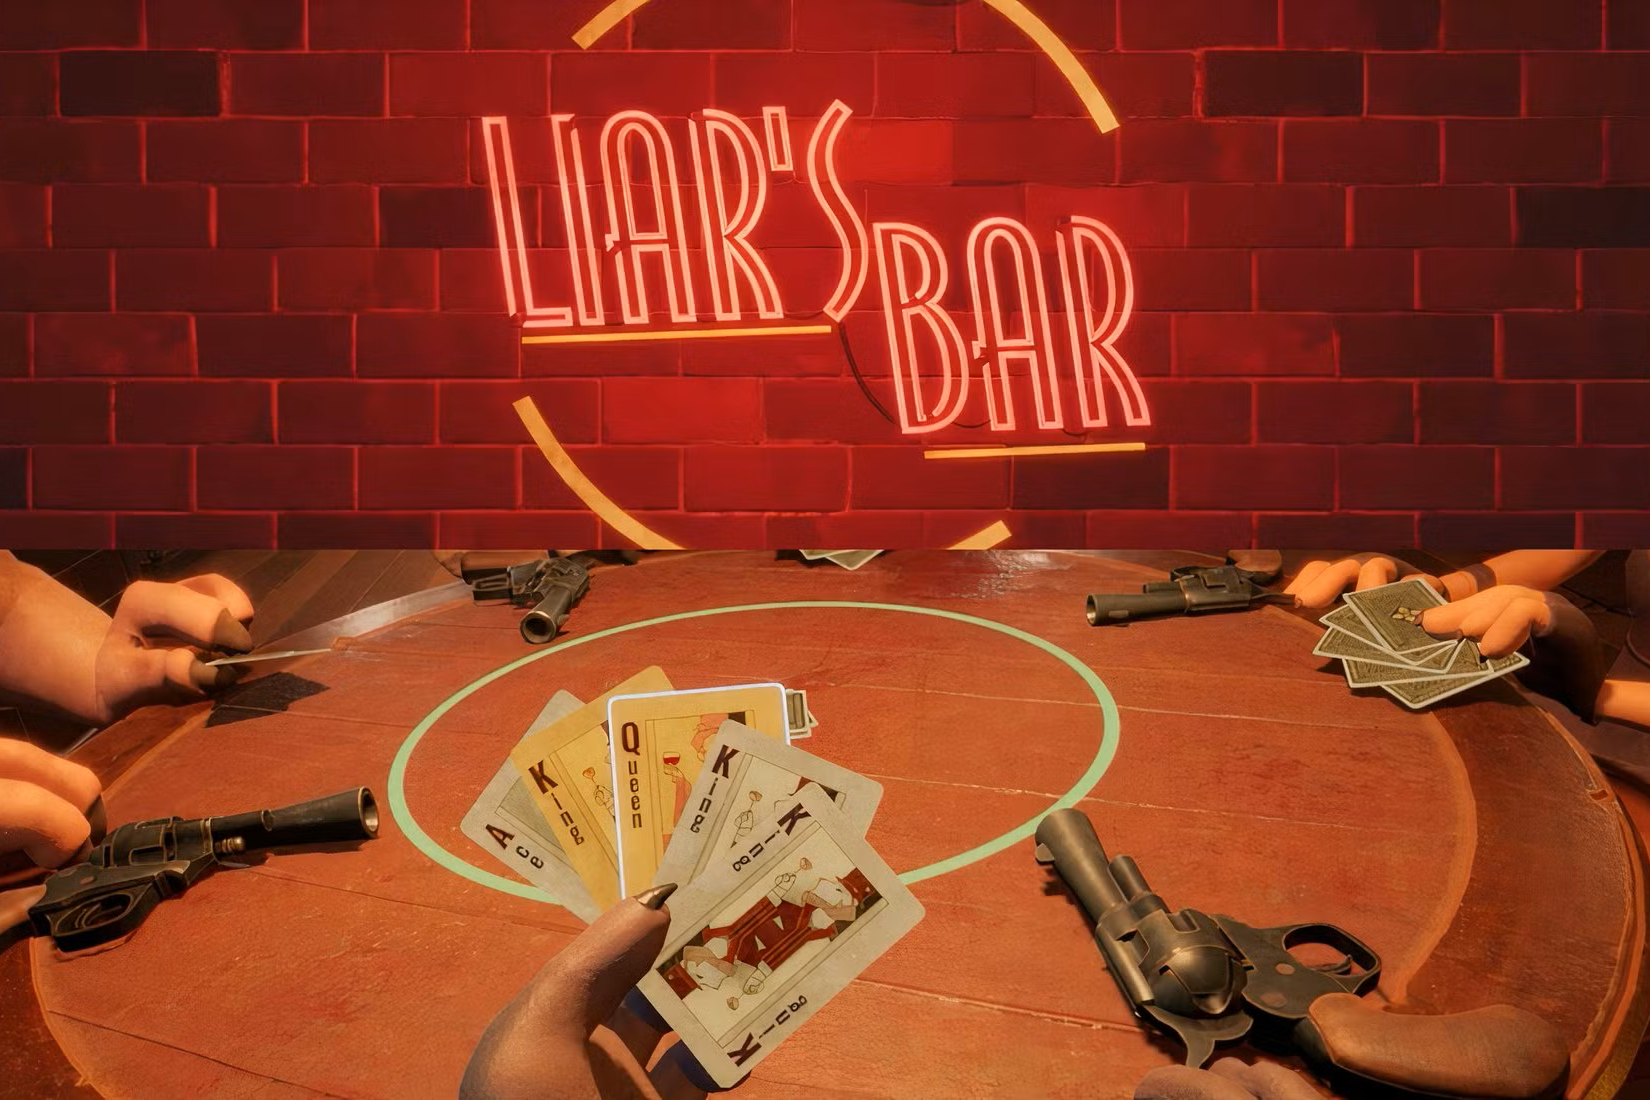
\includegraphics[width=0.9\linewidth]{img/liarsbar.png}
        % \caption{Enter Caption}
        \label{fig:liarsbar}
    \end{figure}
\end{columns}
\end{frame}


\begin{frame}
\frametitle{Các Game Tiêu Biểu Trên Thị Trường}
\begin{columns}
    \column{0.6\textwidth}
    \textbf{Sự Thành Công Của Dòng Game Social \& Party:}
    
    \begin{itemize}
        \item \textbf{Among Us (Social Deduction):}
        \begin{itemize}
            \item Trở thành hiện tượng toàn cầu với lối chơi suy luận đơn giản nhưng kịch tính.
            \item Thành công nhờ tạo ra các tình huống tương tác xã hội "dở khóc dở cười".
        \end{itemize}
        
        \item \textbf{Liar's Bar (Psychological Tabletop):}
        \begin{itemize}
            \item Gây sốt nhờ kết hợp sự căng thẳng của trò chơi "Bluffing" với môi trường 3D sống động.
            \item Đạt thành công lớn trong việc mô phỏng áp lực tâm lý giữa những người chơi trực tiếp.
        \end{itemize}
        
        \item \textbf{Party Animals (Highly Interactive Social):}
        \begin{itemize}
            \item Thu hút hàng triệu người chơi nhờ sự hài hước từ tương tác vật lý.
            \item Thành công nhờ đồ họa 3D bắt mắt và tính giải trí nhóm cực cao.
        \end{itemize}
    \end{itemize}

    \column{0.4\textwidth}
    \centering
    
    \begin{figure}
        \centering
        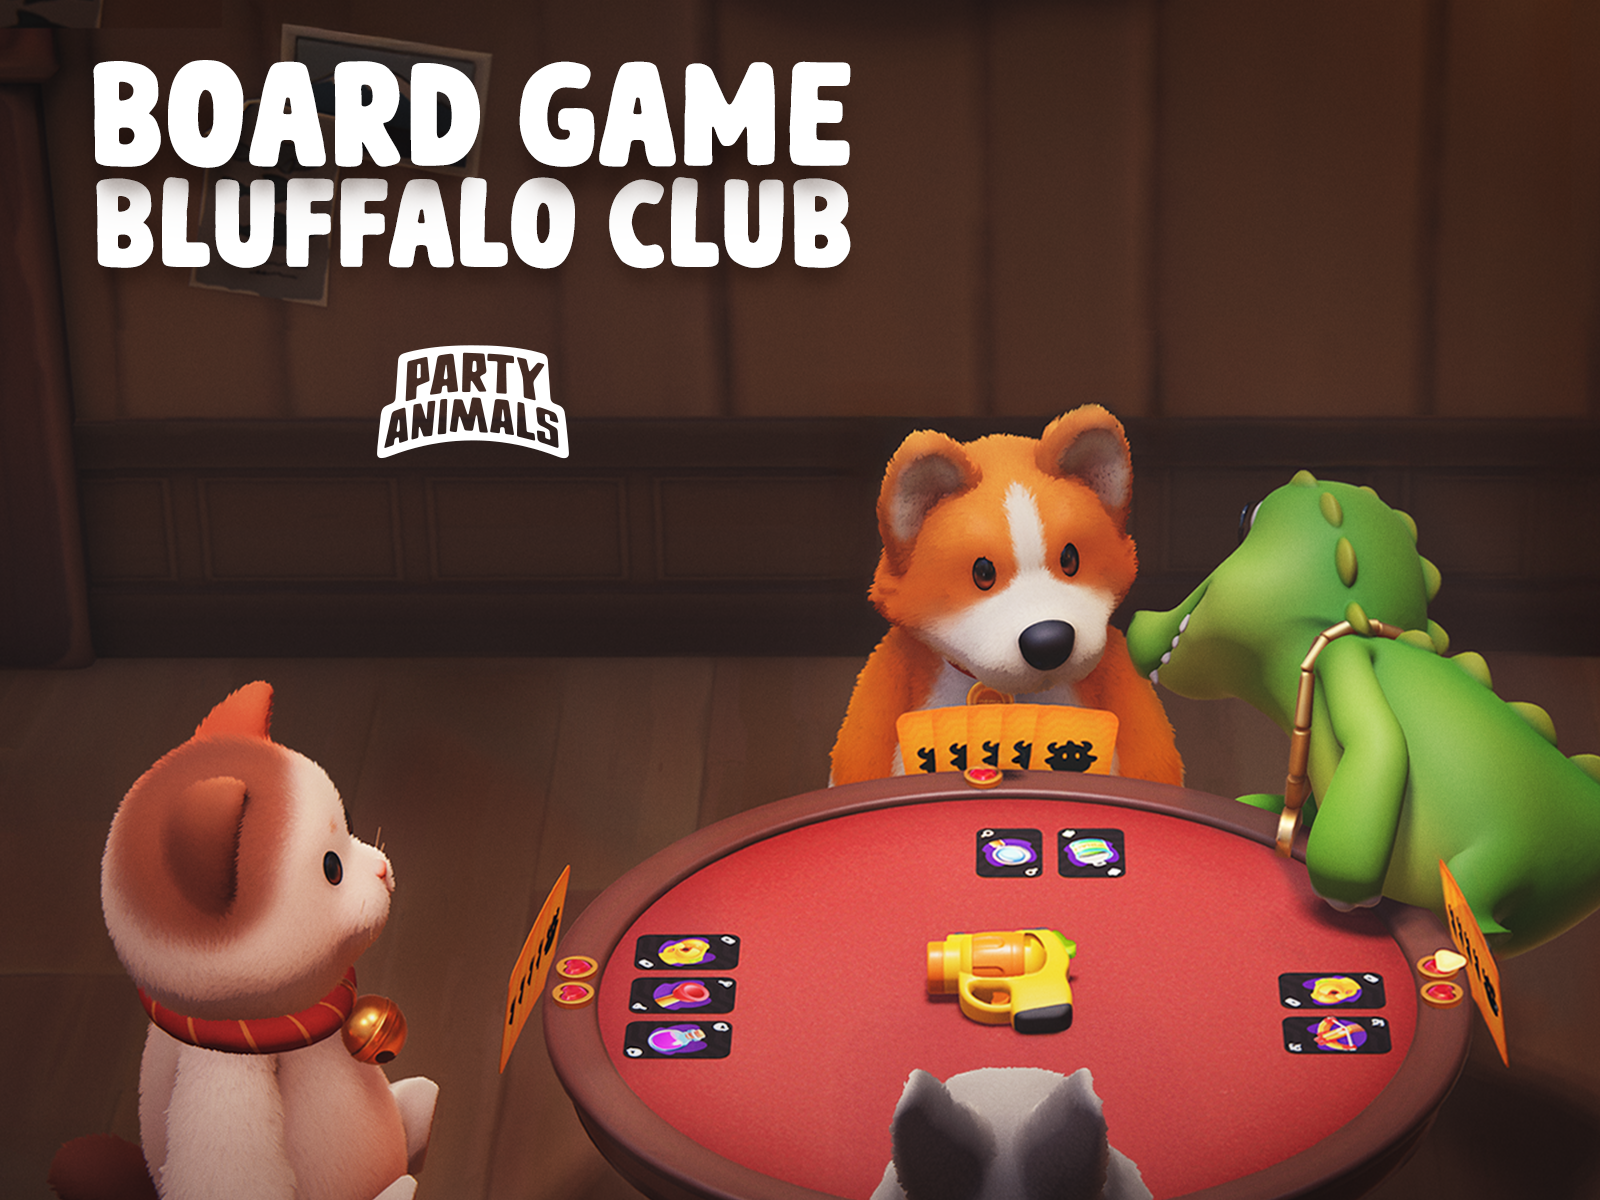
\includegraphics[width=0.9\linewidth]{img/party-animals.png}
        % \caption{Enter Caption}
        \label{fig:animals}
    \end{figure}
\end{columns}
\end{frame}

\begin{frame}
\frametitle{Các Game Tiêu Biểu Trên Thị Trường}
\begin{columns}
    \column{0.6\textwidth}
    \textbf{Sự Thành Công Của Dòng Game Social \& Party:}
    
    \begin{itemize}
        \item \textbf{Among Us (Social Deduction):}
        \begin{itemize}
            \item Trở thành hiện tượng toàn cầu với lối chơi suy luận đơn giản nhưng kịch tính.
            \item Thành công nhờ tạo ra các tình huống tương tác xã hội "dở khóc dở cười".
        \end{itemize}
        
        \item \textbf{Liar's Bar (Psychological Tabletop):}
        \begin{itemize}
            \item Gây sốt nhờ kết hợp sự căng thẳng của trò chơi "Bluffing" với môi trường 3D sống động.
            \item Đạt thành công lớn trong việc mô phỏng áp lực tâm lý giữa những người chơi trực tiếp.
        \end{itemize}
        
        \item \textbf{Party Animals (Highly Interactive Social):}
        \begin{itemize}
            \item Thu hút hàng triệu người chơi nhờ sự hài hước từ tương tác vật lý.
            \item Thành công nhờ đồ họa 3D bắt mắt và tính giải trí nhóm cực cao.
        \end{itemize}
    \end{itemize}

    \column{0.4\textwidth}
    \centering
    
    \vspace{0.5em}
    \begin{block}{Chìa khóa thành công}
        Sự kết hợp giữa \textbf{Tương tác xã hội} + \textbf{Cảm xúc mạnh} + \textbf{Tính giải trí cao}.
    \end{block}
\end{columns}

\end{frame}

% SLIDE 3.1: Cảm Hứng: Saboteur
% \begin{frame}
% \frametitle{Saboteur}
% \begin{itemize}
%     \item \textbf{Luật chơi cốt lõi:}
%     \begin{itemize}
%         \item Phe \textbf{Thợ mỏ (Gold-Diggers)}: Cố gắng nối đường hầm từ điểm xuất phát đến kho báu.
%         \item Phe \textbf{Phá hoại (Saboteurs)}: Bí mật ngăn cản thợ mỏ mà không bị phát hiện.
%     \end{itemize}
%     \item \textbf{Cơ chế:} Đặt thẻ đường, dùng thẻ hành động (phá, sửa, xem map) và \textit{bluffing} (đánh lừa).
%     \item \textbf{Trang bị trong bộ Saboteur}
%     \begin{itemize}
%       \item 40 Thẻ đường (path cards): gồm 31 thẻ thông, 9 thẻ cụt
%       \item 27 Thẻ hành động (action cards)
%       \item 11 Thẻ vai trò (role cards)
%     \end{itemize}
% \end{itemize}
% \end{frame}

\begin{frame}
\frametitle{Cảm Hứng: Saboteur - Trò Chơi Suy Luận Xã Hội Cổ Điển}
\begin{columns}
    % Cột 1: Nội dung và Tương tác (0.55 width)
    \column{0.55\textwidth}
    \textbf{Tính Hấp Dẫn \& Tương Tác:}
    \begin{itemize}
        \item \textbf{Ẩn vai trò (Hidden Roles):} Người chơi không biết ai là Saboteur cho đến phút cuối.
        \item \textbf{Tương tác trực tiếp:} Dùng thẻ hành động để phá hoại công cụ của đối thủ hoặc sửa chữa cho đồng đội.
        \item \textbf{Cơ chế \textit{Bluffing}:} Khả năng đánh lừa, đổ lỗi và thuyết phục là chìa khóa chiến thắng.
    \end{itemize}
    
    % \textbf{Luật Chơi Cơ Bản:}
    % \begin{itemize}
    %     \item Phe \textbf{Thợ mỏ (Gold-Diggers)}: Cố gắng nối đường hầm từ điểm xuất phát đến kho báu.
    %     \item Phe \textbf{Phá hoại (Saboteurs)}: Bí mật ngăn cản thợ mỏ bằng cách đặt thẻ bế tắc hoặc phá hủy đường đi.
    % \end{itemize}
    
    \textbf{Đánh Giá Từ Cộng Đồng (BGG):}
    \begin{itemize}
        \item \textbf{Độ khó:} 1.3/5
        % (Rất dễ tiếp cận, luật chơi đơn giản).
        \item \textbf{Độ lừa lọc: Cao} 
        % \textit{Cực cao} – Linh hồn của trò chơi.
        \item \textbf{Thời gian chơi:} 30 - 45 phút 
        % (Nhanh, phù hợp cho tiệc tùng).
        \item \textbf{Số lượng người chơi:} 3 - 10 người 
        % (Tương tác càng cao khi càng đông).
        % \item \textbf{Độ hấp dẫn:} 7.0/10
        % (Trò chơi "nhập môn" kinh điển).
    \end{itemize}
    % Cột 2: Hình ảnh (0.45 width)
    \column{0.45\textwidth}
    \centering
    \begin{figure}
        \centering
        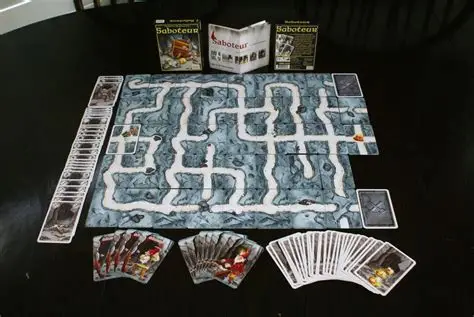
\includegraphics[width=0.9\linewidth]{img/saboteur.png}
        % \caption{Enter Caption}
        \label{fig:placeholder}
    \end{figure}

    % \captionof{figure}{Mô phỏng Board Game Saboteur}
\end{columns}
\end{frame}

% SLIDE 4: Giải Pháp: Fishy Business
\begin{frame}
\frametitle{Mục Tiêu: Fishy Business}
\begin{columns}
    \column{0.5\textwidth}
    \textbf{1. Hiện thực game}
    \begin{itemize}
        \item Số hóa toàn bộ luật chơi: chia bài, kiểm tra đường đi, tính điểm tự động.
        \item Loại bỏ sự rườm rà của việc thiết lập (setup) thủ công.
    \end{itemize}
    \vspace{0.8em} % Tăng khoảng cách một chút để thoáng bài
    \textbf{2. Môi trường 3D}
    \begin{itemize}
        \item Không gian Cabin 3D sống động, tối ưu hóa trải nghiệm thị giác.
        \item Người chơi có Avatar, có thể di chuyển và biểu cảm thời gian thực.
    \end{itemize}

    \column{0.5\textwidth}
    \textbf{3. Multiplayer}
    \begin{itemize}
        \item Kết nối nhiều người chơi thông qua mạng Network.
        \item Tích hợp Voice-Text Chat giúp giao tiếp và "biện minh" trực tiếp.
    \end{itemize}
    \vspace{0.8em}
    \textbf{4. Giải trí bổ trợ}
    \begin{itemize}
        \item Giải quyết "thời gian chết" bằng các hoạt động bên lề thú vị.
        \item Chơi nhạc cụ ảo (piano, guitar), thay đổi trang phục linh hoạt.
    \end{itemize}
\end{columns}
\end{frame}

% SLIDE 5: So Sánh Với Đối Thủ
% \begin{frame}
% \frametitle{Các Game Có Mặt Trên Thị Trường}
% \begin{table}
% \centering
% \begin{tabular}{|l|c|c|c|}
%     \hline
%     \textbf{Tiêu chí} & \textbf{Tabletop Simulator} & \textbf{Board Game Arena} & \textbf{Fishy Business (Project)} \\
%     \hline
%     \textbf{Nền tảng} & PC (Sandbox) & Web (2D) & PC (3D App) \\
%     \hline
%     \textbf{Luật chơi} & Thủ công (Tự tính) & Tự động & Tự động hoàn toàn \\
%     \hline
%     \textbf{Đồ họa} & 3D (Mô phỏng vật lý) & 2D Tĩnh & 3D Social Hub \\
%     \hline
%     \textbf{Tương tác} & Voice chat & Text chat & Avatar, Nhạc cụ, Voice \\
%     \hline
% \end{tabular}
% \end{table}
% \end{frame}
